% Created 2015-02-24 Tue 23:58
\documentclass[11pt]{article}
\usepackage[utf8]{inputenc}
\usepackage{lmodern}
\usepackage[T1]{fontenc}
\usepackage{fixltx2e}
\usepackage{graphicx}
\usepackage{longtable}
\usepackage{float}
\usepackage{wrapfig}
\usepackage{rotating}
\usepackage[normalem]{ulem}
\usepackage{amsmath}
\usepackage{textcomp}
\usepackage{marvosym}
\usepackage{wasysym}
\usepackage{amssymb}
\usepackage{amsmath}
\usepackage[version=3]{mhchem}
\usepackage[numbers,super,sort&compress]{natbib}
\usepackage{natmove}
\usepackage{url}
\usepackage{minted}
\usepackage{underscore}
\usepackage[linktocpage,pdfstartview=FitH,colorlinks,
linkcolor=blue,anchorcolor=blue,
citecolor=blue,filecolor=blue,menucolor=blue,urlcolor=blue]{hyperref}
\usepackage{attachfile}
\usepackage[left=1in, right=1in, top=1in, bottom=1in, nohead]{geometry}
\usepackage{fancyhdr}
\usepackage{hyperref}
\usepackage{setspace}
\usepackage[labelfont=bf]{caption}
\usepackage{amsmath}
\usepackage{enumerate}
\usepackage[parfill]{parskip}
\usepackage[version=3]{mhchem}
\date{Due: 2 March 2015}
\title{}
\begin{document}

\title{Homework 4\\Lectures 5: Potential Energy Sufaces\\(CBE 60553)}
\author{Prof.\ William F.\ Schneider}
\maketitle

In this assignment you will determine some of the properties of \textbf{acetaldehyde} (\ce{CH3CHO}), its isomer \textbf{vinyl alcohol} (\ce{H2C=CH(OH)}), and the \textbf{transtion state} (TS) that interconverts the two:

\begin{center}
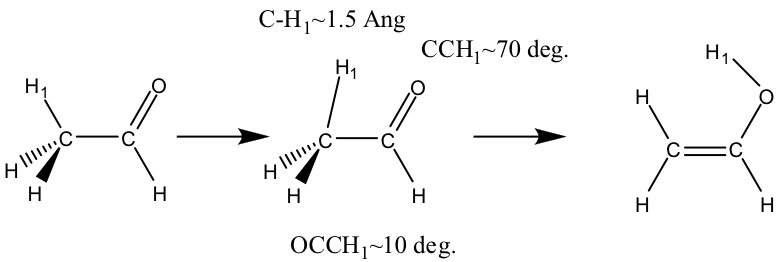
\includegraphics[width=.9\linewidth]{fig1.png}
\end{center}



\section{Characterizing the reactant and product}
\label{sec-1}

\begin{enumerate}[(a)]
\item First, optimize the structures of the reactant acetaldehyde and product vinyl alcohol at the Hartree-Fock level with the 6-31G(d) basis set. Make a table of the key internal coordinates in the two (note you will figure out the TS below):
\end{enumerate}

\begin{center}
\begin{tabular}{llll}
\hline
 & Acetaldehyde & Transition State & Vinyl alcohol\\
\hline
H$_{\text{1}}$–C (\AA{}) &  &  & \\
C–C (\AA{}) &  &  & \\
C–O (\AA{}) &  &  & \\
O-H$_{\text{1}}$ (\AA{}) &  &  & \\
\hline
\end{tabular}
\end{center}

\begin{enumerate}[(b)]
\item Which geometry optimization method did you use in (a)? What type of coordinate system? What were the convergence criteria?
\end{enumerate}

\begin{enumerate}[(c)]
\item Calculate the vibrational spectra of the reactant and product. Confirm that both are true minima (if not, adjust and recalculate). Identify the most prominent (intense) infrared vibrational modes in the two. Could you distinguish these two by their vibrational spectra?
\end{enumerate}

\begin{enumerate}[(d)]
\item Perform single-point energy calculations on the reactant and product at the MP2/6-31G(d) level.  Use the results to complete the table below:
\end{enumerate}

\begin{center}
\begin{tabular}{lll}
\hline
 & Product $-$ reactant  (kJ/mol) & TS $-$ reactant (kJ/mol)\\
\hline
HF/6-31G(d) &  & \\
MP2/6-31G(d) &  & \\
ZPE &  & \\
MP2 + ZPE &  & \\
\hline
\end{tabular}
\end{center}

\begin{enumerate}[(e)]
\item From the frequency calculations on the reactant and product, extract \( H^{\circ}(298)-H(0) \) for each.  Combine with the MP2 + ZPE results to estimate the 298 K reaction enthalpy.
\end{enumerate}

\section{Transition state by scanning}
\label{sec-2}
\begin{enumerate}[(a)]
\item Do a rigid scan about the H$_{\text{1}}$-C-C-O dihedral in acetaldehyde. It is easiest to do this using a z-matrix representation of acetaldehyde. Construct a z-matrix based on your optimized acetaldehyde structure and do a series of energy evaluations as you vary the dihedral angle. Approximately how large is the barrier to rotation about the C–C bond, in kJ/mol?
\end{enumerate}


Recall the z-matrix looks like:

\begin{verbatim}
C1
C2 1 dCC
O  1 dCO  2 aOCC
H1 2 dCH1 1 aHCC1 3 dHCCO

...
\end{verbatim}


\section{Transition state optimization}
\label{sec-3}
\begin{enumerate}[(a)]
\item Guess a structure near the transition state that connects acetaldehyde to vinyl alcohol (note I gave you some hints in the figure) and compute the Hessian at the HF/6-31G(d) level to make sure you are near a saddle point.  Once you have a satisfactory guess, search from this starting point for the transition state. Make sure your calculation converges, and calculate the vibrational spectrum again to make sure you landed at the saddle point. Add the key internal coordinates to the Table in 1(a).

\item What is the magnitude of the imaginary vibrational mode at the transition state?

\item Perform a single-point MP2/6-31G(d) calculations on this transition state. Add the results to the Table in 1(c).

\item Use transition state theory to estimate the rate constant for this reaction at 298 K.  From the frequency calculations on the reactant and transition state, extract \(G^{\circ}(298 K)- G( K) \) for each.  Combine these results with the MP2 + ZPE energies to estimate \( \Delta G^{\ddagger}(298) \).  Evaluate the rate constant using the TST expression:
\end{enumerate}
\begin{equation}
 k(T) =\frac{k_{B} T}{h} e^{-\Delta G^{\ddagger}(T)/k_{B}T}

\section{Bronsted-Evans-Polanyi relations}
\label{sec-4}

Your colleague wants to know if replacing one of the methyl H’s with an F will speed-up or slow down the isomerization. You know from experience that it is much easier to calculate relative rates than absolute ones.
\begin{enumerate}[(a)]
\item Perform additional calculations to determine whether the reaction is more or less exothermic with the F substituent.

\item Perform additional calculations to determine whether the reaction barrier is higher or lower with the F substituent.

\item Do your answers to (a) and (b) conform to expectations from the BEP relationship?
\end{enumerate}

\section{Useful Templates}
\label{sec-5}

\subsection{Frequency calculation:}
\label{sec-5-1}
\begin{verbatim}
$CONTRL SCFTYP=RHF RUNTYP=HESSIAN $END
$BASIS GBASIS=N31 NGAUSS=6 NDFUNC=1 $END
$FORCE METHOD=ANALYTIC VIBANL=.TRUE. $END
$GUESS GUESS=MOREAD NORB=xxx $END ! use if you have a converged SCF wavefunction to read in
$DATA
...
$END
\end{verbatim}


\subsection{Geometry optimization using redundant internal coordinates:}
\label{sec-5-2}
\begin{verbatim}
$CONTRL SCFTYP=RHF RUNTYP=OPTIMIZE NZVAR=”3n-6” $END
$BASIS GBASIS=N31 NGAUSS=6 NDFUNC=1 $END
$STATPT NSTEP=xx $END
$ZMAT DLC=.TRUE. AUTO=.TRUE. $END
$GUESS GUESS=MOREAD NORB=xxx $END ! use if you have a converged SCF wavefunction to read in
$DATA
 ...
$END
$VEC ! converged SCF wavefunction, if you have it
...
$END
\end{verbatim}


\subsection{Transition state search:}
\label{sec-5-3}
\begin{verbatim}
$CONTRL SCFTYP=RHF RUNTYP=SADPOINT NZVAR=”3n-6” $END
$BASIS GBASIS=N31 NGAUSS=6 NDFUNC=1 $END
$STATPT HESS=READ NSTEP=xx $END
$ZMAT DLC=.TRUE. AUTO=.TRUE. $END
$GUESS GUESS=MOREAD NORB=xxx $END ! use if you have a converged SCF wavefunction to read in
$DATA
...
$END
$HESS
...
$END
$VEC
...
$END
\end{verbatim}


\subsection{MP2 calculation:}
\label{sec-5-4}

\begin{verbatim}
$CONTRL SCFTYP=RHF RUNTYP=ENERGY MPLEVL=2 $END
$BASIS GBASIS=N31 NGAUSS=6 NDFUNC=1 $END
$DATA !
...
$END
\end{verbatim}


\subsection{CIS calculation:}
\label{sec-5-5}

\begin{verbatim}
$CONTRL SCFTYP=RHF RUNTYP=ENERGY CITYP=CIS $END
$BASIS GBASIS=N31 NGAUSS=6 NDFUNC=1 $END
$DATA !
...
$END
\end{verbatim}
% Emacs 25.0.50.1 (Org mode 8.2.10)
\end{document}